% 測定機器実装




\section{測定機器1の実装}
はじめに,ESP32-C6 と SCD41 を用いた最小構成のプロトタイプとして,ブレッドボード上に ESP32-C6,SCD41,およびプッシュボタンのみを接続した試作機を作成した(図\ref{fig:Device0}).本プロトタイプは,CO$_2$ 濃度の測定およびサーバへのデータ送信が可能であるかを確認することを目的としている.この試作により,ESP32-C6 と SCD41 間の I$^2$C 通信による CO$_2$ 濃度測定,ならびに Wi-Fi 通信を用いた測定データのサーバ送信が正常に行えることを確認した.これらの結果を踏まえ,本構成を基に測定機器1を作成した.
測定機器1(図\ref{fig:Finishingmachine})は,ESP32-C6(Wi-Fi 通信機能を搭載したマイクロコントローラ),SCD41(CO$_2$ センサ),プッシュボタン,およびリチウムポリマバッテリから構成されている.ESP32-C6 と SCD41 は I$^2$C 通信によって接続されており,ESP32-C6 が測定タイミングの制御およびデータ処理を行う.プッシュボタンは,図〜に示すように抵抗を用いたプルアップ回路として構成しており,ボタンが押されたタイミングで CO$_2$ 濃度の測定およびサーバへのデータ送信を実行する.測定および通信処理が完了した後,ESP32-C6 は DeepSleep モードへ移行し,消費電力を抑える構成とした.DeepSleep の詳細な動作については後述する.動作確認は,まず USB 給電によって行い,その後 ESP32-C6 裏面に実装されたリチウムポリマバッテリ用ソケットにバッテリを接続した状態でも正常に動作することを確認した.なお,測定機器1の外形寸法は,約 40\,mm × 60\,mm である.

\begin{figure}[htbp]
  \centering
  \begin{subfigure}{0.4\linewidth}
    \centering
    \includegraphics[width=\linewidth]{figures/IMG_9311}
    \caption{プロトタイプ}
    \label{fig:Device0}
  \end{subfigure}
  \hfill
  \begin{subfigure}{0.4\linewidth}
    \centering
    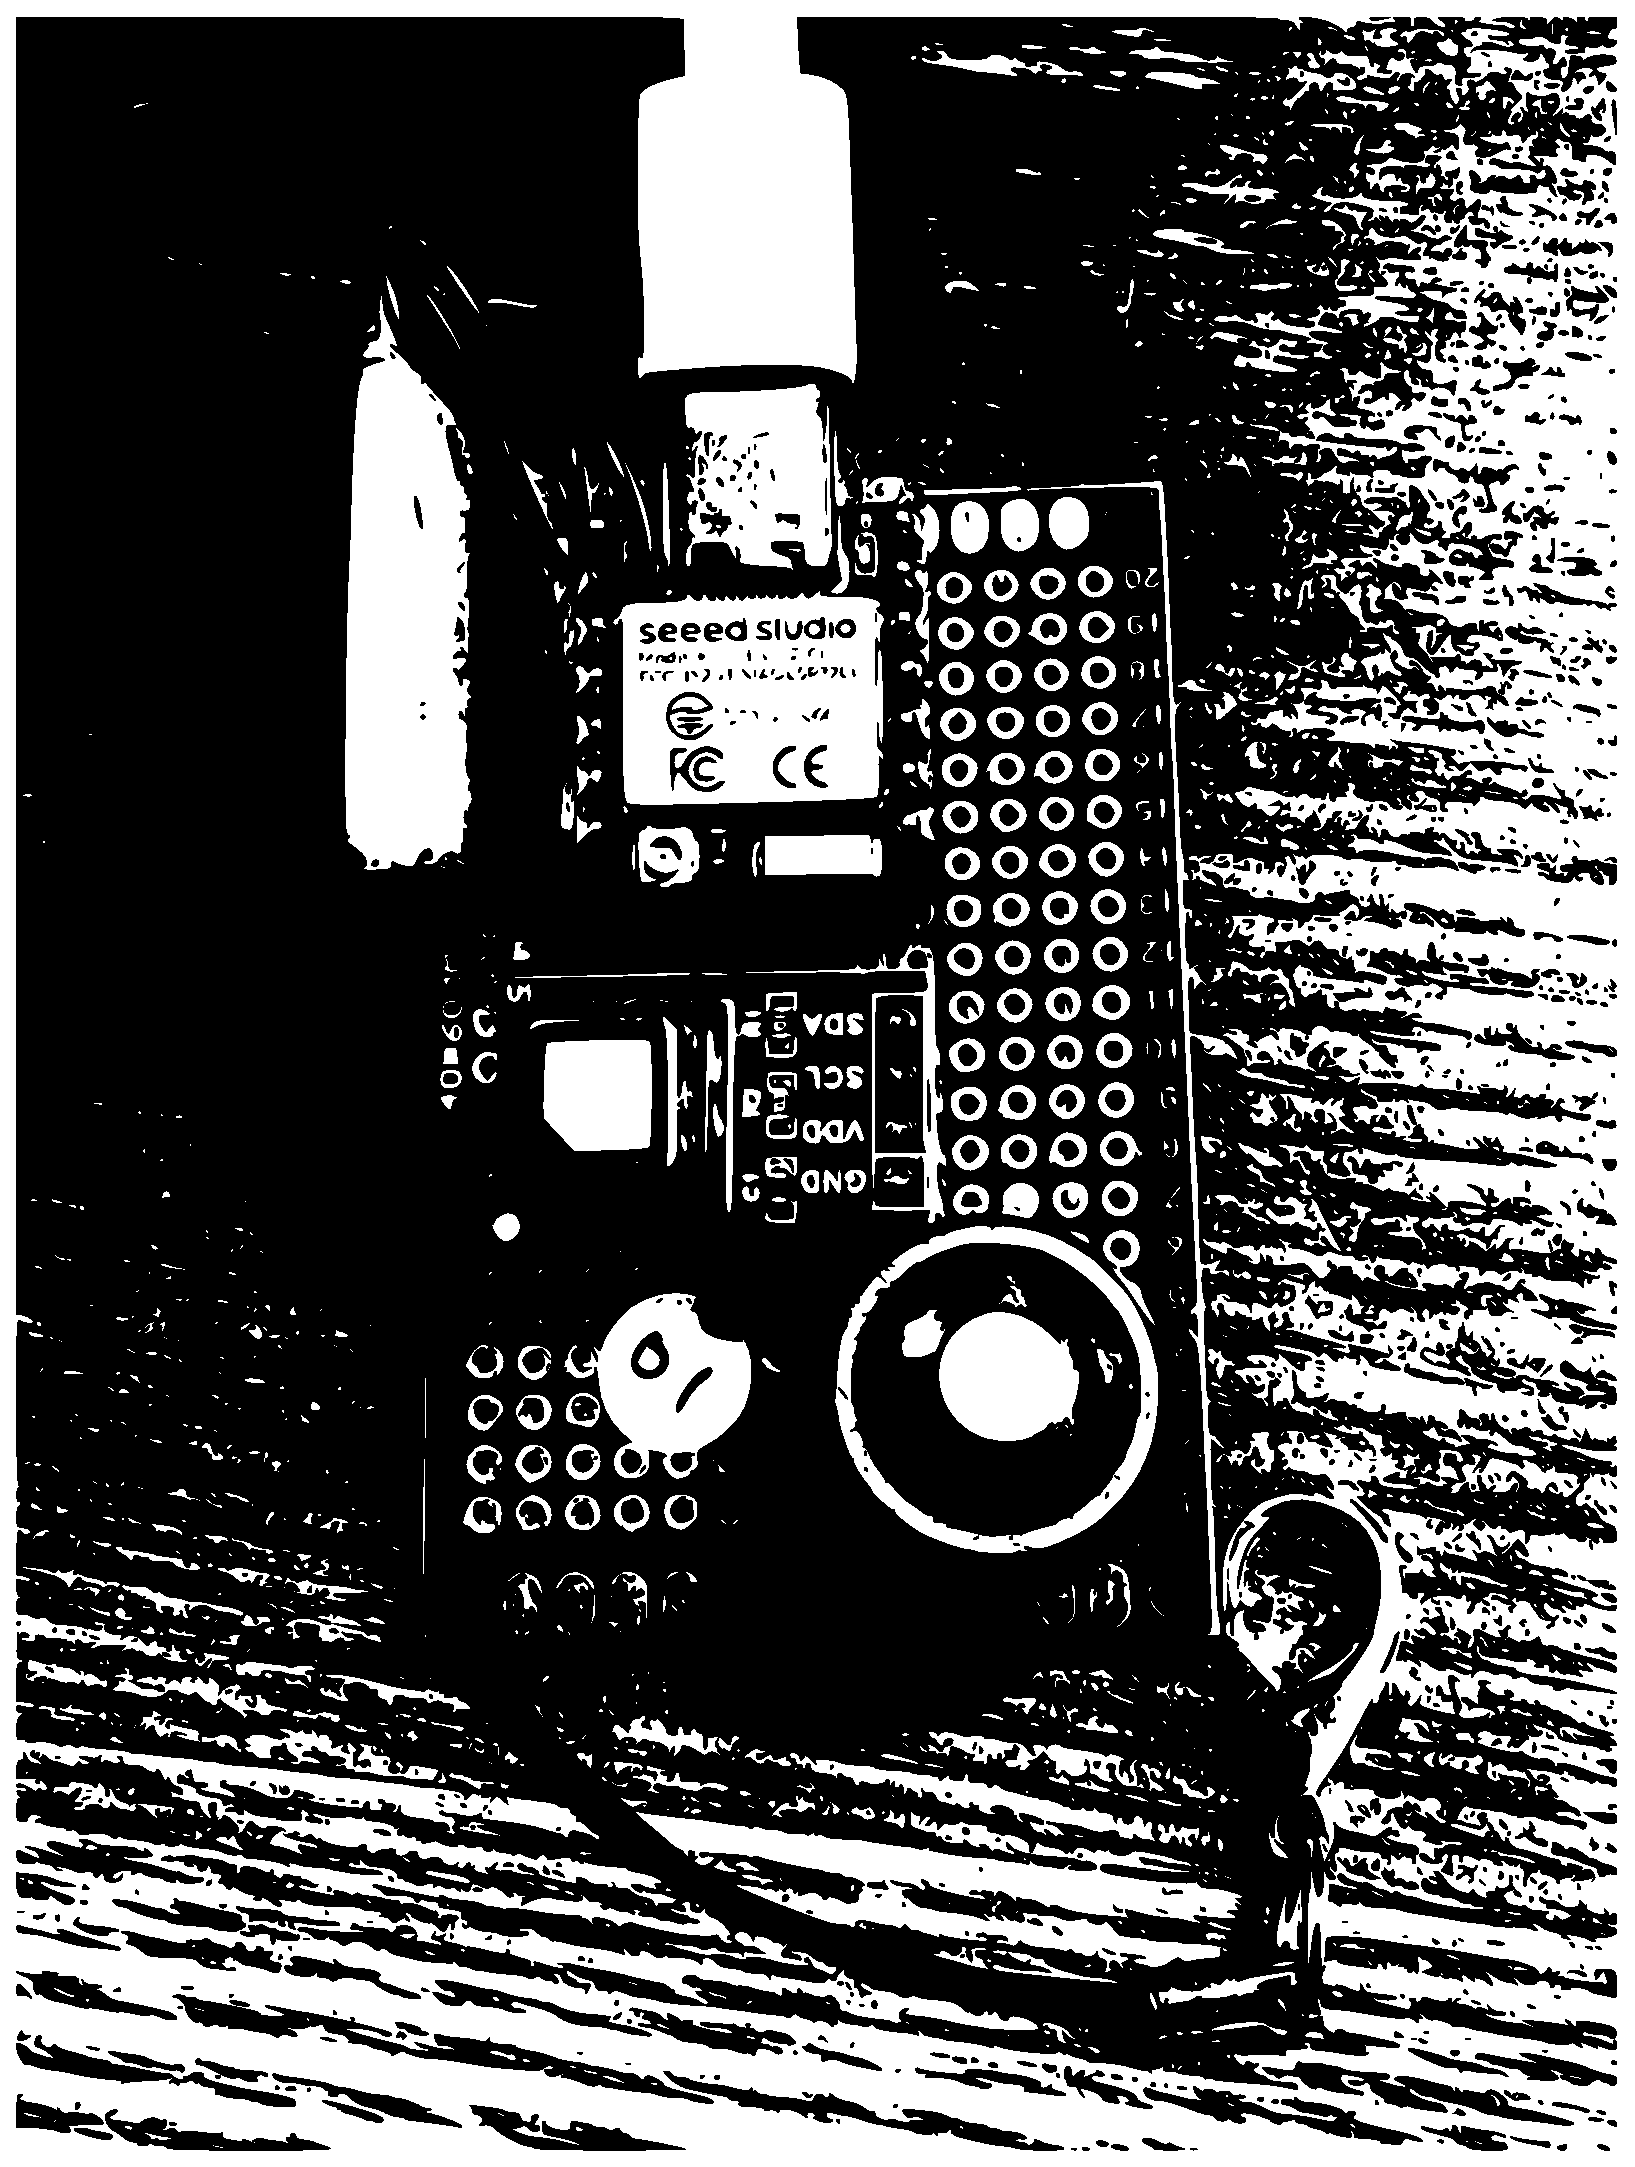
\includegraphics[width=\linewidth]{figures/sisakuki_1}
    \caption{測定機器1}
    \label{fig:Finishingmachine}
  \end{subfigure}
  \caption{プロトタイプおよび測定機器1の外観}
  \label{fig:Device1looks}
\end{figure}

\FloatBarrier





\section{測定機器2,3の実装}
測定機器2は,測定機器1の基本構成を維持したまま,利用者への視覚的なフィードバックを目的として LED を追加した試作機である(図\ref{fig:Device3}).本機器では,測定した CO$_2$ 濃度に応じて LED の色を変化させることで,数値を直接確認しなくても換気状態を把握できる仕組みを実装した.また,本機器は Wi-Fi 通信を用いて測定データをサーバへ送信する構成であるため,屋外環境で使用する場合にはスマートフォンのテザリング等を利用する必要がある.そこで,ESP32-C6 とスマートフォンを Bluetooth 接続し,スマートフォンから SSID およびパスワードを ESP32-C6 に登録する機能を実装した.これにより,利用環境に応じて複数の Wi-Fi ネットワークへ接続可能な構成とした.測定機器2の外形寸法は,約 50\,mm × 70\,mm である.

測定機器3は,測定機器2の機能を維持したまま,携帯性の向上を目的として筐体の小型化を行った試作機である(図\ref{fig:Device3}).ESP32-C6 の表面および裏面の両方に部品を配置する構成とすることで,部品配置の高密度化を図った.その結果,測定機器1と比較してサイズを大幅に縮小することができた.

測定機器3の外形寸法は,約 30\,mm × 40\,mm である.この小型化により,日常生活において持ち運びやすい測定機器を実現した.
\begin{figure}[htbp]
  \centering
  \begin{subfigure}{0.45\linewidth}
    \centering
    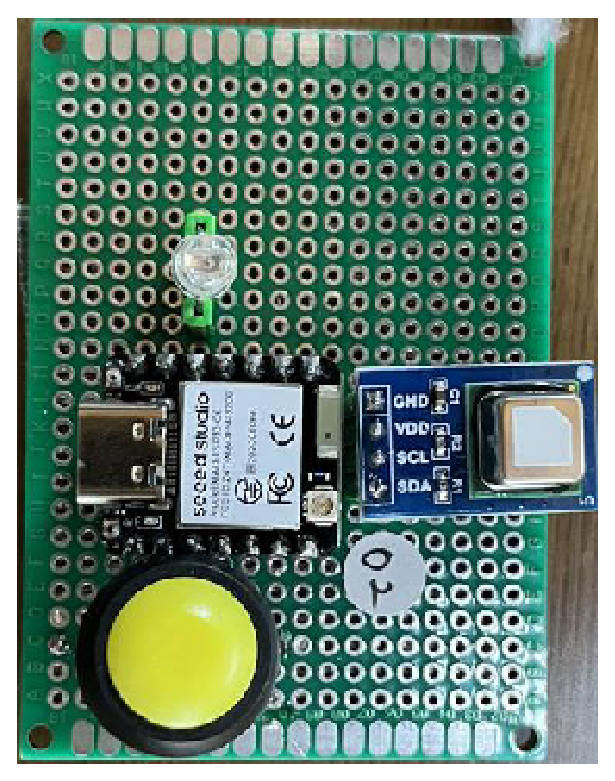
\includegraphics[width=\linewidth]{figures/Image (21)}
    \caption{測定機器2}
    \label{fig:Device2}
  \end{subfigure}
  \hfill
  \begin{subfigure}{0.45\linewidth}
    \centering
    \includegraphics[width=\linewidth]{figures/buttontuki}
    \caption{測定機器3}
    \label{fig:Finishingmachine}
  \end{subfigure}
  \caption{測定機器2および測定機器3の外観}
  \label{fig:Device3}
\end{figure}

\FloatBarrier

\section{測定機器3の課題}
一方で,測定機器3では,Bluetooth 接続やスマートフォンのテザリング設定など,利用者に対して事前の操作や設定を要求する点が課題として明らかになった.特に,高齢者や子どもといった情報機器の操作に不慣れな利用者にとっては,設定作業が負担となる可能性がある.
また,利用環境によっては Wi-Fi 接続が不安定となる場合があり,通信の信頼性という点でも課題が残った.これらの点から,より簡便かつ安定した通信方式の導入が必要であると考えられた.

\section{LTE通信方式の検討}
前節で述べた課題を解決するため,Wi-Fi 環境に依存しない通信方式としてセルラー通信の導入を検討した.セルラー通信を用いることで,屋内外を問わず安定した通信が可能となり,利用者による事前設定を不要とすることが期待できる.本研究では,低消費電力で IoT 用途に適した LTE 通信方式に着目し,LTE 通信を用いた測定機器の開発を行った.

\section{測定機器4の実装}
測定機器4では,測定機器2および3で課題となった通信方式の問題を解決するため,LTE 通信モジュールである SIM7080G を搭載した.(図\ref{fig:sample})これにより,Wi-Fi 環境やスマートフォンのテザリングに依存せず,測定機器単体でサーバへのデータ送信が可能となった.本構成では,利用者が通信設定を行う必要がなくなり,操作負担を大幅に軽減できる.その結果,高齢者や子どもを含む幅広い利用者にとって扱いやすい CO$_2$ 測定機器の実現が可能となった.

\begin{figure}[H]
  \centering


  \begin{subfigure}{0.45\linewidth}
    \centering
    \includegraphics[height=\linewidth,angle=-90]{./figures/LTE-prototype}
    \caption{LTEを使用した試作機}
    \label{fig:LTE-prototype}
  \end{subfigure}

  \vspace{5mm} 
  
  \begin{subfigure}{0.45\linewidth}
    \centering
    \includegraphics[width=\linewidth]{./figures/LTE-ESP-front}
    \caption{測定機器4表面}
    \label{fig:LTE-ESP-front}
  \end{subfigure}
  \hfill
  \begin{subfigure}{0.45\linewidth}
    \centering
    \includegraphics[width=\linewidth]{./figures/LTE-ESP-back}
    \caption{測定機器4裏面}
    \label{fig:LTE-ESP-back}
  \end{subfigure}

  \caption{LTEを使用した測定機器}
  \label{fig:sample}
\end{figure}
\FloatBarrier

\section{DeepSleep を用いた省電力制御}

本研究で開発した CO$_2$ 測定デバイスは,携帯型デバイスとして長時間動作することが求められるため,消費電力の低減が重要な設計要件となる.そこで,本研究では ESP32-C6 が備えるDeepSleep 機能を用いた省電力制御を採用した.DeepSleep とは,マイクロコントローラの動作を一時的に停止し,必要最小限の回路のみを動作させる低消費電力モードである.この状態では,CPU や無線通信機能などが停止されるため,通常動作時と比較して消費電力を大幅に削減することが可能である.

測定機器1〜3では,通常時は DeepSleep 状態とし,ユーザがボタンを押した際にDeepSleep 状態から復帰する構成とした.復帰後は CO$_2$ 濃度の測定を行い,測定データをサーバへ送信した後,再び DeepSleep 状態へ移行する.このような動作により,測定および通信を行う時間を最小限に抑え,バッテリ消費を抑制している.以上の構成により,リチウムポリマーバッテリによる駆動においても,携帯型 CO$_2$ 測定デバイスとして実用的な動作時間を確保することが可能となった.

\section{LTE 通信を用いたデータ送信}

測定機器3では,セルラー通信モジュールである SIM7080G を用いてLTE 回線によるデータ通信を行っている.SIM7080G は,LTE 回線を利用したデータ通信が可能なモジュールであり,広い通信エリアを有することから,屋内外を問わず安定した通信を行うことができる.

測定機器3では,ESP32-C6 と SIM7080G を接続し,測定した CO$_2$ 濃度データをLTE 回線を介してサーバへ送信する構成とした.この方式により,Wi-Fi の SSID やパスワードの設定,スマートフォンによるテザリング操作が不要となり,測定機器単体で通信が可能となっている.以上の構成により,測定環境や利用者の通信環境に依存せず,安定した CO$_2$ 濃度データの取得が可能となった.